\documentclass[12pt,a4paper]{article}
\usepackage{preamble}
\usepackage{booktabs}
\usepackage{array}
\usepackage{float} 
\usepackage{amsmath}
\usepackage{tabularx}
\usepackage{longtable}
\usepackage[utf8]{inputenc}
\usepackage[table]{xcolor}
\usepackage{makecell}

\definecolor{tablegreen}{RGB}{52,168,83}
\definecolor{lightgreen}{RGB}{235,247,238}

\renewcommand{\arraystretch}{1.25}

% ------ Metadata ------
\newcommand{\institution}{FHS/Cyberingeniørskolen}
\newcommand{\laboratory}{MIL-INI}
\newcommand{\coursecode}{INGxxx}
\newcommand{\assignmenttype}{PROSJEKTRAPPORT}
\newcommand{\assignmenttitle}{Sikring av bataljonens ugraderte nettverk}
\newcommand{\studentname}{Gruppe 8}
\newcommand{\partnername}{}
\newcommand{\class}{Gruppe 8}
\newcommand{\labdate}{26. mars 2026}
\newcommand{\submissiondate}{\today}  

\begin{document}

% frontpage.tex
\begingroup

% ===== ENDRE DISSE FELTENE =====
\def\ForsideTittel{Bataljonsnett Litauen}
\def\ForsideEmne{ING3508 Militær informasjonsinfrastruktur}
\def\ForsideGruppe{Gruppe 8}
\def\ForsideDato{29.09.2026}
\def\ForsideOrd{FYLL INN}
% ==============================

\begin{titlepage}
    \thispagestyle{empty}
    \setlength{\parindent}{0pt}
    \setlength{\parskip}{0pt}

    % Skrifttypen gjelder bare forsiden.
    \fontfamily{ptm}\selectfont

    \begin{center}
        \vspace*{5.7cm}

        % Bildet ligger i Media-mappen.
        
\includegraphics[width=5.2cm]{../Media/forsidebilde.pdf}
        \par\vspace{0.6cm}

        {\fontsize{40}{46}\selectfont
        \ForsideTittel\par}

        \vspace{0.7cm}

        {\fontsize{22}{27}\selectfont
        \ForsideEmne\par}

        \vspace{1cm}

        {\fontsize{12}{16}\selectfont\bfseries
        \ForsideGruppe\par
        \vspace{0.3cm}
        \ForsideDato\par}
    \end{center}

    \vfill

    {\fontsize{11}{14}\selectfont
    \color{red}ANTALL ORD: \ForsideOrd\par}

\end{titlepage}
\endgroup


\pagenumbering{Roman}
\setcounter{page}{1}

\begingroup
\setlength{\parindent}{0pt}
\setlength{\parskip}{0.8em}

\section*{Sammendrag}

Rapporten presenterer et forslag til forbedring av
bataljonsstridsgruppens ugraderte nettverk i Rukla,
Litauen. Manglende segmentering, kontroll med tilkoblet
utstyr og overvåkning medfører risiko for uønsket tilgang
og driftsavbrudd som kan ramme telefoni, PA-anlegg,
internettilgang, velferdstjenester, og generell opperativ evne.

Designet omfatter sikkerhetssoner, kontrollert
kommunikasjon, beskyttet trafikk mellom bygg og sikker
administrasjon. Logging og overvåkning med felles
tidsgrunnlag skal støtte oppfølging av hendelser.
Tekniske tiltak suppleres med fysisk sikring,
tydelig driftsansvar og rutiner for bruk,
konfigurasjonskontroll og gjenoppretting.

Eksisterende funksjonalitet skal ivaretas med
tilgjengelig utstyr, uten større nyanskaffelser,
økt ressursbehov eller endringer i forbindelsene
levert av det litauiske forsvaret.

Dokumenterte laboratorietester, begrensninger og
gjenstående risiko skal danne grunnlag for S6s
beslutning om eventuell rekonfigurasjon.
Dokumentasjonen skal også støtte opplæring og
overføring av driftsansvar til fremtidige kontingenter.

\par
\endgroup
\clearpage

%TC:ignore
\section*{Forkortelser}
% Krever \usepackage{longtable} i preambelen.
\small
\setlength{\tabcolsep}{6pt}
\rowcolors{2}{lightgreen}{white}
\begin{longtable}{>{\raggedright\arraybackslash}p{3.8cm}>{\raggedright\arraybackslash}p{9.9cm}}
\caption{Forkortelser brukt i rapporten.}
\label{tab:forkortelser}\\
\toprule
\rowcolor{tablegreen}
\color{white}\textbf{Forkortelse} &
\color{white}\textbf{Betydning} \\
\midrule
\endfirsthead

\toprule
\rowcolor{tablegreen}
\color{white}\textbf{Forkortelse} &
\color{white}\textbf{Betydning} \\
\midrule
\endhead

AAA & Authentication, Authorization and Accounting \\
ACL & Access Control List \\
ARP & Address Resolution Protocol \\
BPDU & Bridge Protocol Data Unit \\
DAI & Dynamic ARP Inspection \\
DHCP & Dynamic Host Configuration Protocol \\
DMVPN & Dynamic Multipoint Virtual Private Network \\
DSCP & Differentiated Services Code Point \\
EIGRP & Enhanced Interior Gateway Routing Protocol \\
ERSPAN & Encapsulated Remote Switched Port Analyzer \\
GRE & Generic Routing Encapsulation \\
IDS & Intrusion Detection System \\
IKEv2 & Internet Key Exchange version 2 \\
IP & Internet Protocol \\
IPsec & Internet Protocol Security \\
IPSG & IP Source Guard \\
LACP & Link Aggregation Control Protocol \\
MGMT & Management \\
NAT & Network Address Translation \\
NHRP & Next Hop Resolution Protocol \\
NTP & Network Time Protocol \\
PAT & Port Address Translation \\
QoS & Quality of Service \\
RSPAN & Remote Switched Port Analyzer \\
SPAN & Switched Port Analyzer \\
SSH & Secure Shell \\
STP & Spanning Tree Protocol \\
TACACS+ & Terminal Access Controller Access-Control System Plus \\
VLAN & Virtual Local Area Network \\
VRF & Virtual Routing and Forwarding \\
WAN & Wide Area Network \\
\bottomrule
\end{longtable}
\rowcolors{1}{}{}
\clearpage

\tableofcontents
\clearpage
%TC:endignore

\pagenumbering{arabic}
\setcounter{page}{1}

\section{Introduksjon}

\setlength{\parindent}{0pt}
\setlength{\parskip}{0.8em}
\subsection{Bakgrunn og problemformulering}

Ved overtakelsen av det ugraderte nettverket til
bataljonsstridsgruppen i Rukla, Litauen, avdekkes
mangelfull dokumentasjon og flere sikkerhetssvakheter.
Nettverket understøtter PA-anlegg,
kontorarbeid og velferdstjenester, men mangler
segmentering og tilstrekkelig kontroll med tilkoblet
utstyr. Private rutere med egne DHCP-servere har
allerede ført til ustabilitet.

Fysisk eksponerte nettverksuttak og manglende sentral
overvåkning og logging øker utfordringene med å
forebygge, oppdage og håndtere uønskede hendelser.
Svakhetene medfører risiko for uønsket tilgang og
bortfall av viktige tjenester. Forbedringer må derfor
omfatte både tekniske tiltak, fysisk sikring og
rutiner for bruk og drift.

Rapporten presenterer et forslag til hvordan bataljonsstridsgruppens ugraderte nettverk kan organiseres og sikres innenfor de tilgjengelige ressursene. Arbeidet tar utgangspunkt i følgende problemstilling:

\begin{quote}
    \emph{Hvordan kan bataljonsstridsgruppens ugraderte
    nettverk sikres og organiseres gjennom tekniske,
    fysiske og administrative tiltak, samtidig som
    eksisterende tjenester opprettholdes innenfor
    tilgjengelige ressurser?}
\end{quote}
\clearpage

% Komprimert teorikapittel.
% Beholder kildene og begrepene som brukes videre i design- og diskusjonskapitlene.

\section{Teori}

\subsection{Lag 2 og lokal sikkerhet}

\subsubsection{DHCP Snooping}

DHCP snooping filtrerer DHCP-meldinger på lag 2 ved å skille mellom trusted og untrusted porter. Legitimiteten til DHCP-svar kontrolleres, og svitsjen bygger samtidig en bindingstabell som knytter IP-adresse, MAC-adresse, VLAN og fysisk port. Tabellen kan brukes videre av Dynamic ARP Inspection (DAI) og IP Source Guard (IPSG) \cite{forsvaret_nettverk_rolle1}.
    
\subsubsection{Dynamic ARP Inspection og IP Source Guard}

DAI validerer ARP-trafikk på untrusted porter mot kjente IP-/MAC-bindinger og kan blokkere ugyldige eller forfalskede ARP-meldinger. IPSG kontrollerer på tilsvarende måte kilde-IP mot DHCP snooping-bindinger eller statiske bindinger og reduserer muligheten for IP-spoofing. For statisk adresserte enheter kan egne ARP ACL-er eller statiske bindinger være nødvendig \cite{forsvaret_nettverk_rolle1}.

\subsubsection{Port Security}

Port Security begrenser hvilke eller hvor mange MAC-adresser som kan brukes på en klientport. Ved brudd kan trafikk droppes, hendelsen logges eller porten settes i error-disabled-tilstand avhengig av valgt violation-modus. Mekanismen gir et ekstra lag med kontroll, men erstatter ikke sterk klientautentisering \cite{forsvaret_nettverk_rolle1}.

\subsubsection{Spanning Tree og beskyttelsesmekanismer}

Spanning Tree Protocol (STP) hindrer lag-2-løkker ved å beregne en løkkefri topologi og blokkere redundante veier. STP er relevant også i nettverk uten planlagte redundante lenker fordi feilkobling eller senere endringer kan introdusere løkker \cite{cisco_stp_3850}.

PortFast lar edge-porter gå raskt til forwarding og brukes på porter mot endeenheter. BPDU Guard beskytter slike porter ved å sette dem i error-disabled dersom de mottar uventede BPDUs. Root Guard hindrer at en nedstrøms forbindelse overtar root-rollen, mens Loop Guard hindrer at porter feilaktig går til forwarding dersom forventede BPDUs forsvinner, for eksempel ved en enveis linkfeil \cite{forsvaret_nettverk_rolle1,nsm_n03}.

\subsection{Segmentering og rutet transport}

\subsubsection{VLAN og VRF-Lite}

VLAN segmenterer et fysisk Ethernet-nettverk i separate broadcast-domener. Kommunikasjon mellom VLAN krever ruting, og VLAN alene bestemmer ikke hvilke rutede forbindelser som skal tillates. Dette må styres med for eksempel ACL-er eller brannmurregler.

Virtual Routing and Forwarding (VRF) gjør det mulig å ha flere separate rutingtabeller på samme fysiske ruter eller lag-3-svitsj \cite{forsvaret_nettverk_rolle1}.

\subsubsection{GRE og DMVPN}

Generic Routing Encapsulation (GRE) kapsler trafikk inn i en ny GRE/IP-pakke slik at den kan transporteres gjennom et IP-nettverk. GRE gir ikke i seg selv kryptografisk beskyttelse og kombineres derfor ofte med IPsec \cite{rfc2784,cisco_dmvpn_current}.

Dynamic Multipoint Virtual Private Network (DMVPN) kombinerer mGRE, NHRP og ruting for å opprette dynamiske forbindelser mellom hub- og spoke-rutere. NHRP knytter tunneladresser til underliggende NBMA-adresser og muliggjør dynamiske spoke-to-spoke-forbindelser. I Phase 2 kan spoke etablere direkte forbindelse når rutingen bevarer remote spoke som neste hopp. I Phase 3 kan hub bruke NHRP Redirect og spoke NHRP Shortcut, slik at hub fortsatt kan være rutingens neste hopp samtidig som dataplanet optimaliseres til direkte spoke-to-spoke-trafikk \cite{cisco_dmvpn_current,dmvpn_phase_3}.

\subsubsection{IPsec og IKEv2}

IPsec beskytter IP-trafikk og kan tilby konfidensialitet, integritet og autentisering av datakilde. I DMVPN brukes IPsec ofte som tunnel protection rundt GRE-trafikken. Transportmodus er vanlig fordi GRE allerede kapsler den opprinnelige trafikken \cite{rfc4301,cisco_dmvpn_ipsec_transport}.

IKEv2 brukes til å etablere og vedlikeholde Security Associations (SAs) og kryptografiske nøkler. \texttt{IKE\_SA\_INIT} forhandler algoritmer og nøkkelmateriale, \texttt{IKE\_AUTH} autentiserer partene og etablerer første Child SA, mens \texttt{CREATE\_CHILD\_SA} kan opprette eller fornye ytterligere sikkerhetsforbindelser \cite{rfc7296}.

\subsection{Tilgangskontroll og trafikkstyring}

\subsubsection{ACL}

Access Control Lists (ACL-er) filtrerer trafikk etter regler som kan omfatte kilde- og destinasjons-IP, protokoll og transportlagsport. Regler behandles i rekkefølge, og trafikk som ikke eksplisitt tillates treffes normalt av en implisitt deny \cite{forsvaret_nettverk_rolle1}.

\subsubsection{NAT/PAT}

Port Address Translation (PAT), også kalt NAT overload, gjør det mulig for flere interne klienter å dele en global IPv4-adresse ved å skille forbindelser med blant annet transportlagsporter. PAT reduserer behovet for globale IPv4-adresser, men erstatter ikke eksplisitt tilgangskontroll \cite{cisco_pat}.

\subsubsection{QoS}

Quality of Service (QoS) brukes til å klassifisere, merke og prioritere trafikk. Køhåndtering og båndbreddefordeling kan sikre at viktige tjenester får en definert andel av kapasiteten ved belastning, men QoS skaper ikke mer fysisk båndbredde \cite{cisco_qos}.

\subsubsection{EtherChannel}

EtherChannel kombinerer flere fysiske Ethernet-lenker til en logisk forbindelse. Dette kan gi høyere samlet kapasitet og redundans dersom en medlemslenke faller ut. En enkelt trafikkstrøm bruker normalt en medlemslenke, mens flere strømmer kan fordeles mellom dem. LACP er en standardisert metode for etablering av slike kanaler, mens PAgP er Cisco-proprietær \cite{forsvaret_nettverk_rolle1}.

\subsection{Identitet og administrasjon}

\subsubsection{SSH og AAA}

SSH gir kryptert fjernadministrasjon og er et sikrere alternativ til Telnet, som sender trafikk ukryptert \cite{forsvaret_nettverk_rolle1}.

AAA står for Authentication, Authorization and Accounting. Autentisering bekrefter identitet, autorisasjon bestemmer hvilke handlinger en bruker kan utføre, og accounting registrerer sesjoner og eventuelt kommandoaktivitet for sporbarhet.

\subsubsection{TACACS+}

TACACS+ brukes ofte til administrasjon av nettverksutstyr og skiller autentisering, autorisasjon og accounting i separate prosesser. Protokollen bruker tradisjonelt TCP-port 49. Den delte hemmeligheten beskytter meldingskroppen, men RFC 8907 beskriver mekanismen som obfuskering og ikke sterk kryptografisk beskyttelse. TACACS+ bør derfor brukes over et beskyttet administrasjonsnett eller sammen med egnet transportbeskyttelse \cite{rfc8907}.

\subsubsection{RADIUS og IEEE 802.1X}

RADIUS brukes ofte til nettverkstilgang og sammen med IEEE 802.1X. Tradisjonelt brukes UDP 1812 for autentisering/autorisasjon og UDP 1813 for accounting. RADIUS krypterer ikke hele meldingen, og sikkerheten avhenger blant annet av valgt EAP-metode og transportbeskyttelse \cite{rfc2865,rfc2866,rfc3579}.

IEEE 802.1X gir portbasert tilgangskontroll. Endepunktet fungerer som supplicant, access-svitsjen som authenticator/NAS og RADIUS-klient, og autentiseringsserveren validerer bruker eller enhet. EAPOL kan utveksles mens porten fortsatt er uautorisert, og vanlig datatrafikk tillates først når policyen godkjenner tilgangen \cite{rfc3580,cisco_wired_dot1x}. PEAP kan etablere en TLS-tunnel som beskytter den indre autentiseringen \cite{ms_peap}.

\subsection{Overvåkning og logging}

\subsubsection{Syslog og NTP}

Sentral logging og overvåkning gjør det mulig å korrelere aktivitet fra flere enheter og gir bedre grunnlag for feilsøking og hendelseshåndtering \cite{nsm_n03}. Syslog brukes til å sende hendelser fra nettverksenheter til en sentral loggtjeneste. Konsistent tidsstempling er viktig, og NTP brukes til å synkronisere klokker mellom systemene \cite{nsm_n03}.

\subsubsection{Suricata og Security Onion}

Suricata er en nettverksbasert IDS/IPS-motor som analyserer trafikk og kan generere strukturerte hendelser, blant annet i EVE JSON-format. Security Onion kombinerer blant annet Suricata med logging, nettverksmetadata og analyseverktøy. Ved passiv overvåkning mottar sensoren vanligvis kopiert trafikk fra TAP eller trafikkspeiling \cite{suricata_eve,security_onion_intro}.

\subsubsection{SPAN, RSPAN og ERSPAN}

SPAN speiler trafikk til en lokal monitorport. RSPAN transporterer speilet trafikk gjennom et eget VLAN over lag-2-trunker, mens ERSPAN kapsler trafikken inn i GRE og kan transportere den over et rutet IP-nettverk. Valg av metode avhenger derfor av hvor sensoren er plassert og om trafikken må krysse et lag-2- eller lag-3-nett \cite{cisco_span_rspan_3850,cisco_erspan_3850}.

\subsubsection{SNMPv3}

Simple Network Management Protocol (SNMP) brukes til overvåkning og administrasjon av nettverksenheter gjennom en manager--agent-modell. Manageren kan hente statusdata, mens agentene kan sende traps eller informs. SNMPv3 støtter autentisering og kryptering. Sikkerhetsnivået \texttt{authPriv} gir begge deler \cite{cisco_snmp_security}.

NSM N-03 (2012) anbefaler at SNMP deaktiveres dersom det ikke er nødvendig. Dersom det brukes, beskriver veiledningen blant annet bruk av nyeste versjon, ACL-begrensning til autoriserte administrasjonssystemer, minst mulig rettigheter og autentisering/kryptering. Henvisningen gjelder 2012-utgaven og er ikke en påstand om dagens generelle NSM-krav \cite{nsm_n03}.

\subsection{Automatisering}

\subsubsection{Ansible}

Ansible er et agentløst automatiseringsverktøy som kan brukes til konfigurasjonsstyring, utrulling og sikkerhetskopiering. Control node kjører playbooks mot managed nodes, normalt over SSH. Inventory beskriver hvilke enheter som skal administreres, mens moduler utfører konkrete oppgaver. Playbooks uttrykker ønsket sekvens og tilstand i YAML, og idempotente moduler forsøker å unngå unødvendige endringer ved gjentatte kjøringer. Roller kan brukes for å organisere og gjenbruke automasjon \cite{ansible}.

\clearpage

% Designkapittel. Krever array, longtable, booktabs, float, amsmath,
% graphicx, xcolor med table-opsjon og caption i hoveddokumentet.
% Eksisterende figurstier og tabell-/figurlabels er beholdt.
% K1--K8 erstatter den tidligere nummereringen 1--19.
\begingroup
\captionsetup[table]{justification=centering,singlelinecheck=false}
\section{Design}
Designarbeidet tok utgangspunkt i nettverket S6-seksjonen overtok ved HO/TO. Nettverket var flatt, kontrollen over tilkoblede enheter var begrenset, og det manglet både fjernadministrasjon og sentral overvåkning. Den nye løsningen skulle videreføre UGRADERT telefoni, PA-anlegg og Internett-tilgang for kontorbruk og velferd, men samtidig gi S6 bedre kontroll med administrasjon, overvåkning og gjenoppretting.

Kapitlet beskriver rammebetingelsene og kravene som styrte designet, og forklarer hvorfor de ulike løsningene ble tatt i bruk. Det skilles mellom selve designvalgene, forutsetninger som må være på plass før produksjonssetting, og forhold som må verifiseres gjennom testing. At en mekanisme er inkludert i designet, betyr derfor ikke i seg selv at det tilhørende kravet er oppfylt.

\subsection{Utgangspunkt og rammebetingelser}
Stabssjefen fastsatte, i samråd med S6, følgende rammebetingelser for rekonfigurasjonen. De styrte designarbeidet og ble brukt som føringer når ulike tekniske alternativer måtte vurderes opp mot hverandre:
\begingroup
\small
\setlength{\tabcolsep}{4pt}
\renewcommand{\arraystretch}{1.18}
\captionsetup{justification=centering,singlelinecheck=false}
\begin{longtable}{@{}>{\raggedright\arraybackslash}p{0.08\linewidth} >{\raggedright\arraybackslash}p{0.25\linewidth} >{\raggedright\arraybackslash}p{0.60\linewidth}@{}}
\caption{Rammebetingelser for rekonfigurasjonen.}\label{tab:rammebetingelser}\\
\toprule
\textbf{ID} & \textbf{Rammebetingelse} & \textbf{Beskrivelse} \\
\midrule
\endfirsthead
\toprule
\textbf{ID} & \textbf{Rammebetingelse} & \textbf{Beskrivelse} \\
\midrule
\endhead
\midrule
\multicolumn{3}{r}{Fortsetter på neste side}\\
\endfoot
\bottomrule
\endlastfoot
F1 & Risiko og ressursbruk & Nettverket skal redusere sikkerhetsrisikoen til et akseptabelt nivå, uten at drift og bruk krever mer ressurser enn før rekonfigurasjonen. \\
\addlinespace
F2 & Funksjonalitet & Nettverket skal fortsatt gi samme funksjonalitet for brukerne. \\
\addlinespace
F3 & Anskaffelser & Løsningen skal ikke kreve større nyanskaffelser av maskinvare, programvare eller lisenser. \\
\addlinespace
F4 & Leverandørens forbindelser & Konfigurasjonen til forbindelsene levert av det litauiske forsvaret skal ikke måtte endres. \\
\addlinespace
F5 & Dokumentasjon & Nettverket skal dokumenteres for nåværende og fremtidige kontingenter. \\
\addlinespace
F6 & Godkjenning & Ingen endringer skal gjøres i produksjonsnettet før S6 har akseptert den operative risikoen ved endringene. \\
\end{longtable}
\endgroup

\subsection{Designkrav}
Tabell \ref{tab:designkrav} viser kravene som ble utledet fra svakhetene som kom fram ved HO/TO, sammen med behovet for sikker drift og gjenoppretting. Kravene beskriver hva løsningen skal oppnå, de tekniske og administrative tiltakene er virkemidlene som skal bidra til dette.

Krav som hadde størst betydning for sikkerhet og operativ funksjon fikk prioritet H, mens støttende krav til forvaltning og gjenoppretting fikk prioritet M. Tabellen er sortert med H-kravene først. Prioriteringen følger rammebetingelsene F1--F6. Dersom et krav ikke var dokumentert oppfylt, ble det stående som et uavklart forhold eller som gjenstående risiko.

\begingroup
\small
\setlength{\tabcolsep}{4pt}
\renewcommand{\arraystretch}{1.18}
\captionsetup{justification=centering,singlelinecheck=false}
\begin{longtable}{@{}>{\raggedright\arraybackslash}p{0.055\linewidth} >{\raggedright\arraybackslash}p{0.48\linewidth} >{\raggedright\arraybackslash}p{0.30\linewidth} >{\centering\arraybackslash}p{0.065\linewidth}@{}}
\caption{Prioriterte designkrav og grunnlaget for dem.}\label{tab:designkrav}\\
\toprule
\textbf{ID} & \textbf{Krav} & \textbf{Grunnlag} & \textbf{Pri.} \\
\midrule
\endfirsthead
\toprule
\textbf{ID} & \textbf{Krav} & \textbf{Grunnlag} & \textbf{Pri.} \\
\midrule
\endhead
\midrule
\multicolumn{4}{r}{Fortsetter på neste side}\\
\endfoot
\bottomrule
\endlastfoot
K1 & Tjenester og brukergrupper skal segmenteres etter funksjon og risiko, lokalt og mellom bygg. & Flatt nettverk uten sikkerhetssoner. & H \\
\addlinespace
K2 & Kommunikasjon mellom soner og mot Internett skal begrenses til dokumenterte behov. Trafikk med beskyttelsesbehov skal sikres mot innsyn og manipulering under transport. & Ubegrenset kommunikasjon, utsatte kontorklienter og eksternt administrert transportnett. & H \\
\addlinespace
K3 & Tilgang via nettverksuttak skal kontrolleres. Uautoriserte og feilkonfigurerte enheter skal begrenses fra å forstyrre tjenestene. & Ubeskyttede uttak og hendelser med private DHCP-servere. & H \\
\addlinespace
K4 & Nettverksenheter skal kunne fjernadministreres sikkert av autorisert personell, med sporbar administrativ aktivitet. & Manglende fjernadministrasjon og behov for kontrollert drift. & H \\
\addlinespace
K5 & Hendelser og relevant nettverkstrafikk skal kunne samles inn og analyseres sentralt med felles tidsgrunnlag. & Manglende logginnsamling, sikkerhetsovervåkning og synkroniserte klokker. & H \\
\addlinespace
K6 & Feil og belastning skal håndteres slik at nødvendige tjenester opprettholder avtalte funksjons- og tilgjengelighetsmål. & Operativ betydning for telefoni, PA-anlegg og Internett. Rammebetingelse F2. & H \\
\addlinespace
K7 & Fysisk plassering, bruk og driftsansvar skal redusere risikoen fra ubeskyttede uttak og Internett-klienter i sensitive arbeidsområder. & Uttak utenfor beskyttet område og Internett-klienter i rom med sensitiv aktivitet. & H \\
\addlinespace
K8 & Konfigurasjoner skal dokumenteres, kontrolleres og kunne gjenopprettes til en kjent tilstand. & Rammebetingelsene F1 og F5. Behov for stabil drift, gjenoppretting og kontinuitet ved HO/TO. & M \\
\end{longtable}
\endgroup

Krav-ID-ene ga sporbarhet mellom behov og designvalg og dannet grunnlaget for verifikasjon. For K6 var tjenestespesifikke akseptkriterier en forutsetning for å vurdere resultatene fra belastnings- og feiltester. Kravoppfyllelse måtte underbygges med dokumenterte resultater.

\subsection{IP-adresseringsplan}
Adresseplanen gir tjenestenettene en fast og gjenkjennelig struktur på tvers av lokasjoner, og støtter dermed segmenteringen i K1. Samme navngivning og dokumentasjonsmodell brukes overalt for å gjøre drift og overlevering enklere, i tråd med K8 og F5.

\subsubsection{Lokal nettverksplan}
Tabell \ref{tab:ipplan-site-x} viser adresseplanen for det lokale nettet på lokasjon X. Den samme strukturen brukes på alle lokasjoner, slik at adresseringen blir forutsigbar og enkel å kjenne igjen.

Det lokale adresseområdet er 10.0.0.0/8. Andre oktett angir lokasjon, mens tredje oktett angir tjenestenett. MGMT-nettet på lokasjon 1 blir derfor 10.1.10.0/24, mens det tilsvarende nettet på lokasjon 2 blir 10.2.10.0/24.

Denne oppbygningen gjør det mulig å lese både lokasjon og tjeneste direkte ut fra IP-adressen, samtidig som samme modell kan gjenbrukes når nye lokasjoner legges til.

\begin{table}[H]
    \centering
    \caption{IP-adresseplan for det lokale nettverket på lokasjon X.}
    \label{tab:ipplan-site-x}
    \small
    \renewcommand{\arraystretch}{1.3}
    \setlength{\tabcolsep}{4pt}
    \rowcolors{2}{lightgreen}{white}
    \begin{tabular}{
        >{\bfseries}l
        c
        l
        l
        l
        c
    }
        \toprule
        \rowcolor{tablegreen}
        \color{white}\textbf{VRF} &
        \color{white}\textbf{VLAN} &
        \color{white}\textbf{Nett-ID} &
        \color{white}\textbf{Gateway} &
        \color{white}\textbf{Adresseområde} &
        \color{white}\textbf{Res.} \\
        \midrule
        MGMT       & 10 & 10.X.10.0/24 & 10.X.10.1 & 10.X.10.1--10.X.10.254 & 40 \\
        INET       & 20 & 10.X.20.0/24 & 10.X.20.1 & 10.X.20.1--10.X.20.254 & -- \\
        UNET       & 30 & 10.X.30.0/24 & 10.X.30.1 & 10.X.30.1--10.X.30.254 & -- \\
        PA         & 40 & 10.X.40.0/24 & 10.X.40.1 & 10.X.40.1--10.X.40.254 & -- \\
        MONITORING & 50 & 10.X.50.0/24 & 10.X.50.1 & 10.X.50.1--10.X.50.254 & 40 \\
        \bottomrule
    \end{tabular}
    \rowcolors{1}{}{}
\end{table}
\noindent
Kolonnen \textbf{Res.} angir hvor mange adresser som reserveres utenfor den dynamiske adressepoolen. Dette er spesielt relevant i MGMT- og MONITORING-nettene, hvor nettverksenheter og overvåkningskomponenter benytter faste adresser.

Et /24-nett inneholder 254 brukbare host-adresser. Dersom 40 adresser reserveres, gjenstår:
\[
    A_{\text{ledige}} = 254 - 40 = 214
\]
adresser til øvrig bruk.

Andre oktett brukes som lokasjonsidentifikator. Dersom lokasjons-ID 0 reserveres, kan den lokale adresseplanen benytte ID 1--255. I tunnelplanen 172.16.<tjeneste>.X/24 må X derimot ligge mellom 1 og 254, siden .255 er broadcast-adressen. Tredje oktett identifiserer tjenestenettet og følger samme nummerering på alle lokasjoner.

\subsubsection{Loopback- og DMVPN-plan}
Tabellene \ref{tab:loopback-site-x} og \ref{tab:dmvpn-site-x} viser hvordan segmenteringen videreføres mellom lokasjonene, og hvilke overlay som beskyttes med IPsec. Dette knytter adresse- og tunnelplanen direkte til K1 og K2.

Loopback-adresser brukes fordi de gir stabile endepunkter for administrasjon, ruting og tunnelterminering.

Hver VRF har en ordinær loopback som representerer VRF-en lokalt. I tillegg har hvert DMVPN-overlay en egen global kildeloopback.

Egne kildeloopbacker ga hvert DMVPN-overlay en unik
underlay-kildeadresse. Disse adressene ble brukt i
\texttt{match identity remote address} i de tilhørende
IKEv2-profilene. Dette hindret overlapp mellom overlayenes
adressebaserte matchkriterier og sikret entydig valg av
IKEv2-profil.

Hvert IPsec-beskyttet overlay fikk en egen IKEv2- og
IPsec-profil. Dette la til rette for separate
autentiseringsnøkler og tydeligere skille mellom
sikkerhetsdomenene. Med uavhengige forhåndsdelte nøkler
ville kompromittering av nøkkelen til ett overlay ikke
i seg selv kompromittere autentiseringen i de øvrige.
Separasjonen forenklet også administrasjon og feilsøking.

\begin{table}[H]
    \centering
    \caption{Loopback-adresser benyttet på lokasjon X.}
    \label{tab:loopback-site-x}
    \small
    \renewcommand{\arraystretch}{1.3}
    \setlength{\tabcolsep}{8pt}
    \rowcolors{2}{lightgreen}{white}
    \begin{tabular}{lll}
        \toprule
        \rowcolor{tablegreen}
        \color{white}\textbf{Tjeneste} &
        \color{white}\textbf{VRF-loopback} &
        \color{white}\textbf{DMVPN kildeloopback} \\
        \midrule
        MGMT       & Loopback10 & Loopback11 \\
        INET       & Loopback20 & Loopback21 \\
        UNET       & Loopback30 & Loopback31 \\
        PA         & Loopback40 & Loopback41 \\
        MONITORING & Loopback50 & Loopback51 \\
        \bottomrule
    \end{tabular}
    \rowcolors{1}{}{}
\end{table}

\begin{table}[H]
    \centering
    \caption{DMVPN-adresseplan for lokasjon X.}
    \label{tab:dmvpn-site-x}
    \small
    \renewcommand{\arraystretch}{1.3}
    \setlength{\tabcolsep}{5pt}
    \rowcolors{2}{lightgreen}{white}
    \begin{tabular}{llllcc}
        \toprule
        \rowcolor{tablegreen}
        \color{white}\textbf{Tunnel} &
        \color{white}\textbf{VRF} &
        \color{white}\textbf{Tunnel-IP} &
        \color{white}\textbf{Tunnel source} &
        \color{white}\textbf{NHRP-ID} &
        \color{white}\textbf{IPsec} \\
        \midrule
        Tunnel10 & MGMT       & 172.16.10.X/24 & Loopback11 & 10 & Ja \\
        Tunnel20 & INET       & 172.16.20.X/24 & Loopback21 & 20 & Nei \\
        Tunnel30 & UNET       & 172.16.30.X/24 & Loopback31 & 30 & Ja \\
        Tunnel40 & PA         & 172.16.40.X/24 & Loopback41 & 40 & Ja \\
        Tunnel50 & MONITORING & 172.16.50.X/24 & Loopback51 & 50 & Ja \\
        \bottomrule
    \end{tabular}
    \rowcolors{1}{}{}
\end{table}

\subsubsection{QoS}
QoS skal bidra til at viktige tjenester fortsatt får kapasitet når WAN-forbindelsen er belastet, og støtter dermed K6 og F2. Tabell \ref{tab:qos-site-x} viser vektingen mellom trafikkklassene. Vektingen angir ønsket prioritering, men faktisk kapasitet må fortsatt dokumenteres gjennom belastningstester.

Tjenester med størst operativ betydning får derfor en definert minimumsandel av kapasiteten når WAN-forbindelsen er belastet.

Trafikken klassifiseres etter tjenestenett og merkes med DSCP. Til sammen fordeles 75~\% mellom de definerte trafikkklassene. De resterende 25~\% blir ikke eksplisitt reservert til \texttt{class-default} av generatoren.

For en trafikkklasse $i$ beregnes minimum båndbreddeandel som:
\[
    B_i =
    \frac{P_i}{P_t}
    \cdot 75\%, \quad \text{hvor } P_t = \sum_i P_i
\]
Her er $P_i$ klassens prioriteringsvekt, $P_t$ summen av vektene og $B_i$ den beregnede båndbreddeandelen. Generatoren avrunder først ned til heltall. Resterende prosentpoeng fordeles til klassene med størst desimalrest, ved lik rest prioriteres høyere vekt. Dermed summerer de tildelte andelene til 75 prosent.
\begin{table}[H]
    \centering
    \caption{QoS-vekting og båndbreddefordeling for lokasjon X.}
    \label{tab:qos-site-x}
    \small
    \renewcommand{\arraystretch}{1.3}
    \setlength{\tabcolsep}{7pt}
    \rowcolors{2}{lightgreen}{white}
    \begin{tabular}{lccc}
        \toprule
        \rowcolor{tablegreen}
        \color{white}\textbf{VRF} &
        \color{white}\textbf{DSCP} &
        \color{white}\textbf{Vekt ($P_i$)} &
        \color{white}\textbf{Båndbreddeandel ($B_i$)} \\
        \midrule
        MGMT          & AF21 & 5  & 11\% \\
        INET          & AF11 & 2  & 4\%  \\
        UNET          & AF42 & 7  & 16\% \\
        PA            & AF41 & 10 & 22\% \\
        MONITORING    & AF43 & 10 & 22\% \\
        Ufordelt andel & --   & -- & 25\% \\
        \bottomrule
    \end{tabular}
    \rowcolors{1}{}{}
\end{table}
\noindent
Fordelingen favoriserer operative tjenester og overvåkning når forbindelsen er presset. Generatoren bruker VLAN som grunnlag for klassifisering og DSCP for plassering i køklasser. Velferds- og Internett-trafikk får lavere prioritet fordi redusert ytelse der har mindre operativ konsekvens.

\subsection{Fysisk design}
Figur \ref{fig:physical-design} viser den fysiske oppkoblingen. Løsningen bygger på eksisterende utstyr i tråd med F3, samtidig som redundans og tilgjengelighet ivaretas der det er mulig (K6). Fysisk sikring og kontroll med nettverksuttak må håndteres i tillegg (K7).

Det fysiske designet viser hvordan rutere, svitsjer, servere og endepunkter kobles sammen på hver lokasjon.

Hver lokasjon består av en lokasjonsruter, en distribusjonssvitsj og én eller flere aksessvitsjer. De lokale VLAN-ene transporteres frem til ruteren, som fungerer som lag-3-grense mellom tjenestenettene og DMVPN-overlayene.

Der portkapasiteten tillater det, brukes EtherChannel mellom svitsjene. Det gir redundans dersom én fysisk lenke faller ut og gjør det mulig å utnytte kapasiteten i flere parallelle forbindelser.

\begin{figure}[H]
    \centering
    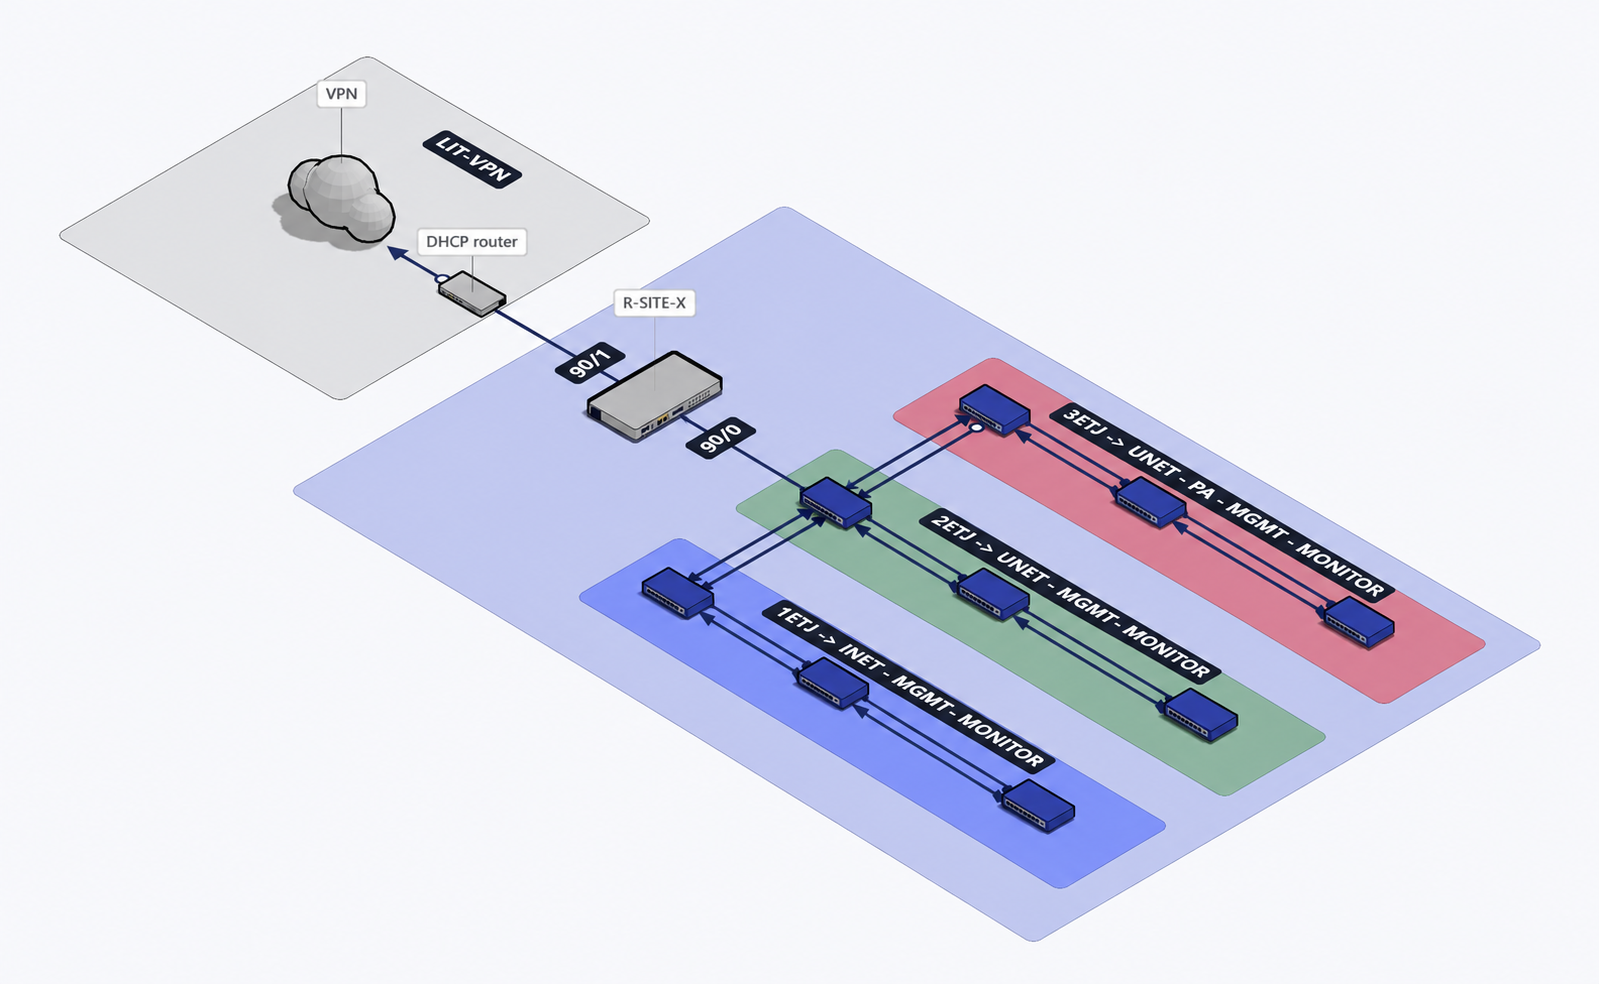
\includegraphics[width=1\textwidth]{../Media/bygg_nettverk.png}
    \caption{Fysisk oppkobling av enheter i lokasjonsstrukturen.}
    \label{fig:physical-design}
\end{figure}

\subsection{DMVPN Phase 3-arkitektur}
Figur \ref{fig:logisk_arkitektur_dmvpn} viser hvordan tjenestene og segmenteringen videreføres mellom bygg uten å kreve endringer i leverandørens transportnett. Arkitekturen ivaretar dermed F2, K1 og rammebetingelsen i F4.

BNHQ på lokasjon 1 fungerer som DMVPN-hub og NHRP Next Hop Server (NHS). De øvrige lokasjonene er spokes og registrerer seg mot hubben.

Kontrollplanet følger en hub-and-spoke-modell for registrering og dynamisk ruting. Dataplanet kan derimot etablere direkte forbindelser mellom spokes, slik at trafikken ikke trenger å fortsette via hubben når en snarvei først er opprettet.

I Phase 3 sender hubben NHRP Redirect, mens spoke-ruterne bruker NHRP Shortcut. Den første trafikken kan dermed gå via hubben, før det etableres en direkte spoke-to-spoke-forbindelse.

Dette reduserer unødvendig trafikk gjennom BNHQ og gjør det enklere å legge til nye lokasjoner uten å opprette et komplett sett med statiske punkt-til-punkt-tunneler.
\begin{figure}[H]
    \centering
    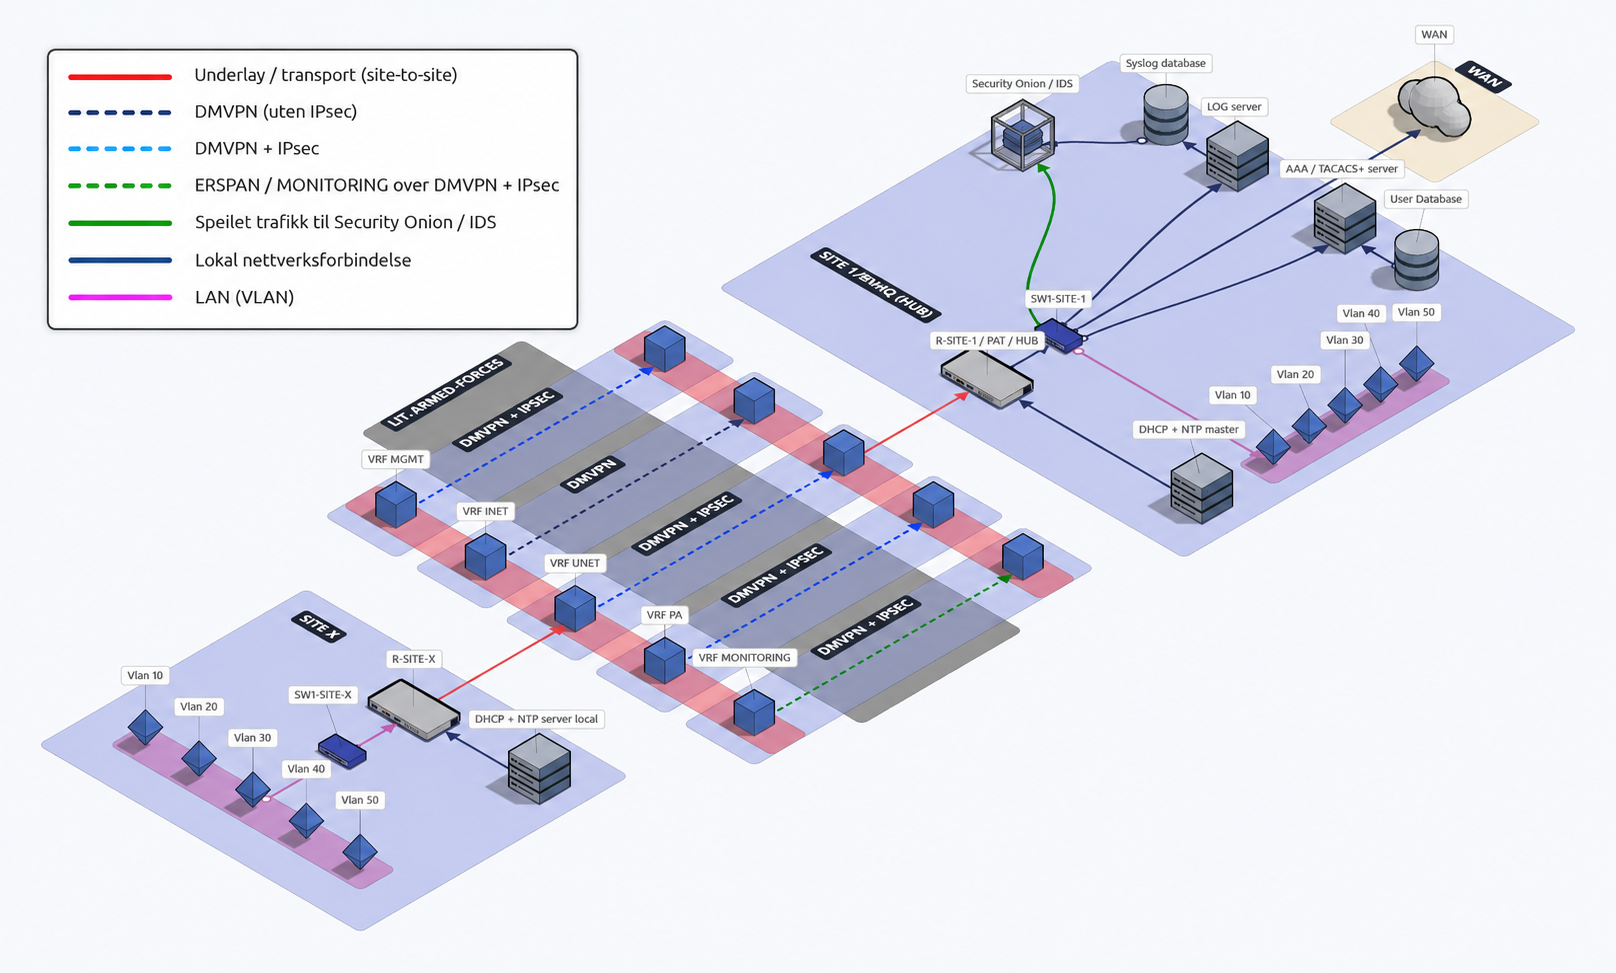
\includegraphics[width=1\textwidth]{../Media/logisk_arkitektur.png}
    \caption{DMVPN Phase 3-arkitektur mellom hub og spoke-lokasjoner.}
    \label{fig:logisk_arkitektur_dmvpn}
\end{figure}
\noindent
DMVPN-overlayet bruker det eksisterende lag-3-VPN-et fra det litauiske forsvaret som transportnett, slik at leverandørkonfigurasjonen kan stå uendret (F4). Dette forutsetter at transportnettet har nødvendig ruting og slipper gjennom tunneltrafikken. Ruting, filtrering og MTU må derfor verifiseres før produksjonssetting.

Overlay med behov for konfidensialitet og integritet beskyttes med IPsec (K2). Dermed er trafikken beskyttet også når den går gjennom infrastruktur som eFP ikke administrerer.

BNHQ samler de sentrale tjenestene, blant annet TACACS+, syslog, NTP og Security Onion, i tillegg til tilkoblingen mot sivil ISP.

\subsection{Logisk design}
VLAN skiller tjenestene lokalt, mens VRF-Lite og separate overlay viderefører segmenteringen på lag 3 og mellom lokasjonene (K1). Kommunikasjon som skal tillates mellom soner styres av en eksplisitt trafikkpolicy (K2).

Figur \ref{fig:logisk_ip} viser den logiske arkitekturen på et spoke-site. Klienter og tjenester ble fordelt på VLAN etter funksjon. VLAN-ene ble lagt til lokasjonsruteren, med hvert lag-3-grensesnitt tilordnet den tilhørende VRF-en.

MGMT, INET, UNET, PA og MONITORING ligger i hver sin VRF og har dermed separate rutingtabeller. Trafikk mellom sonene krever en eksplisitt definert sammenkobling og tilhørende trafikkpolicy.

Hver VRF har sitt eget DMVPN-overlay mellom lokasjonene. Slik beholdes segmenteringen over WAN-et, selv om overlayene bruker det samme underliggende transportnettet.

\begin{figure}[H]
    \centering
    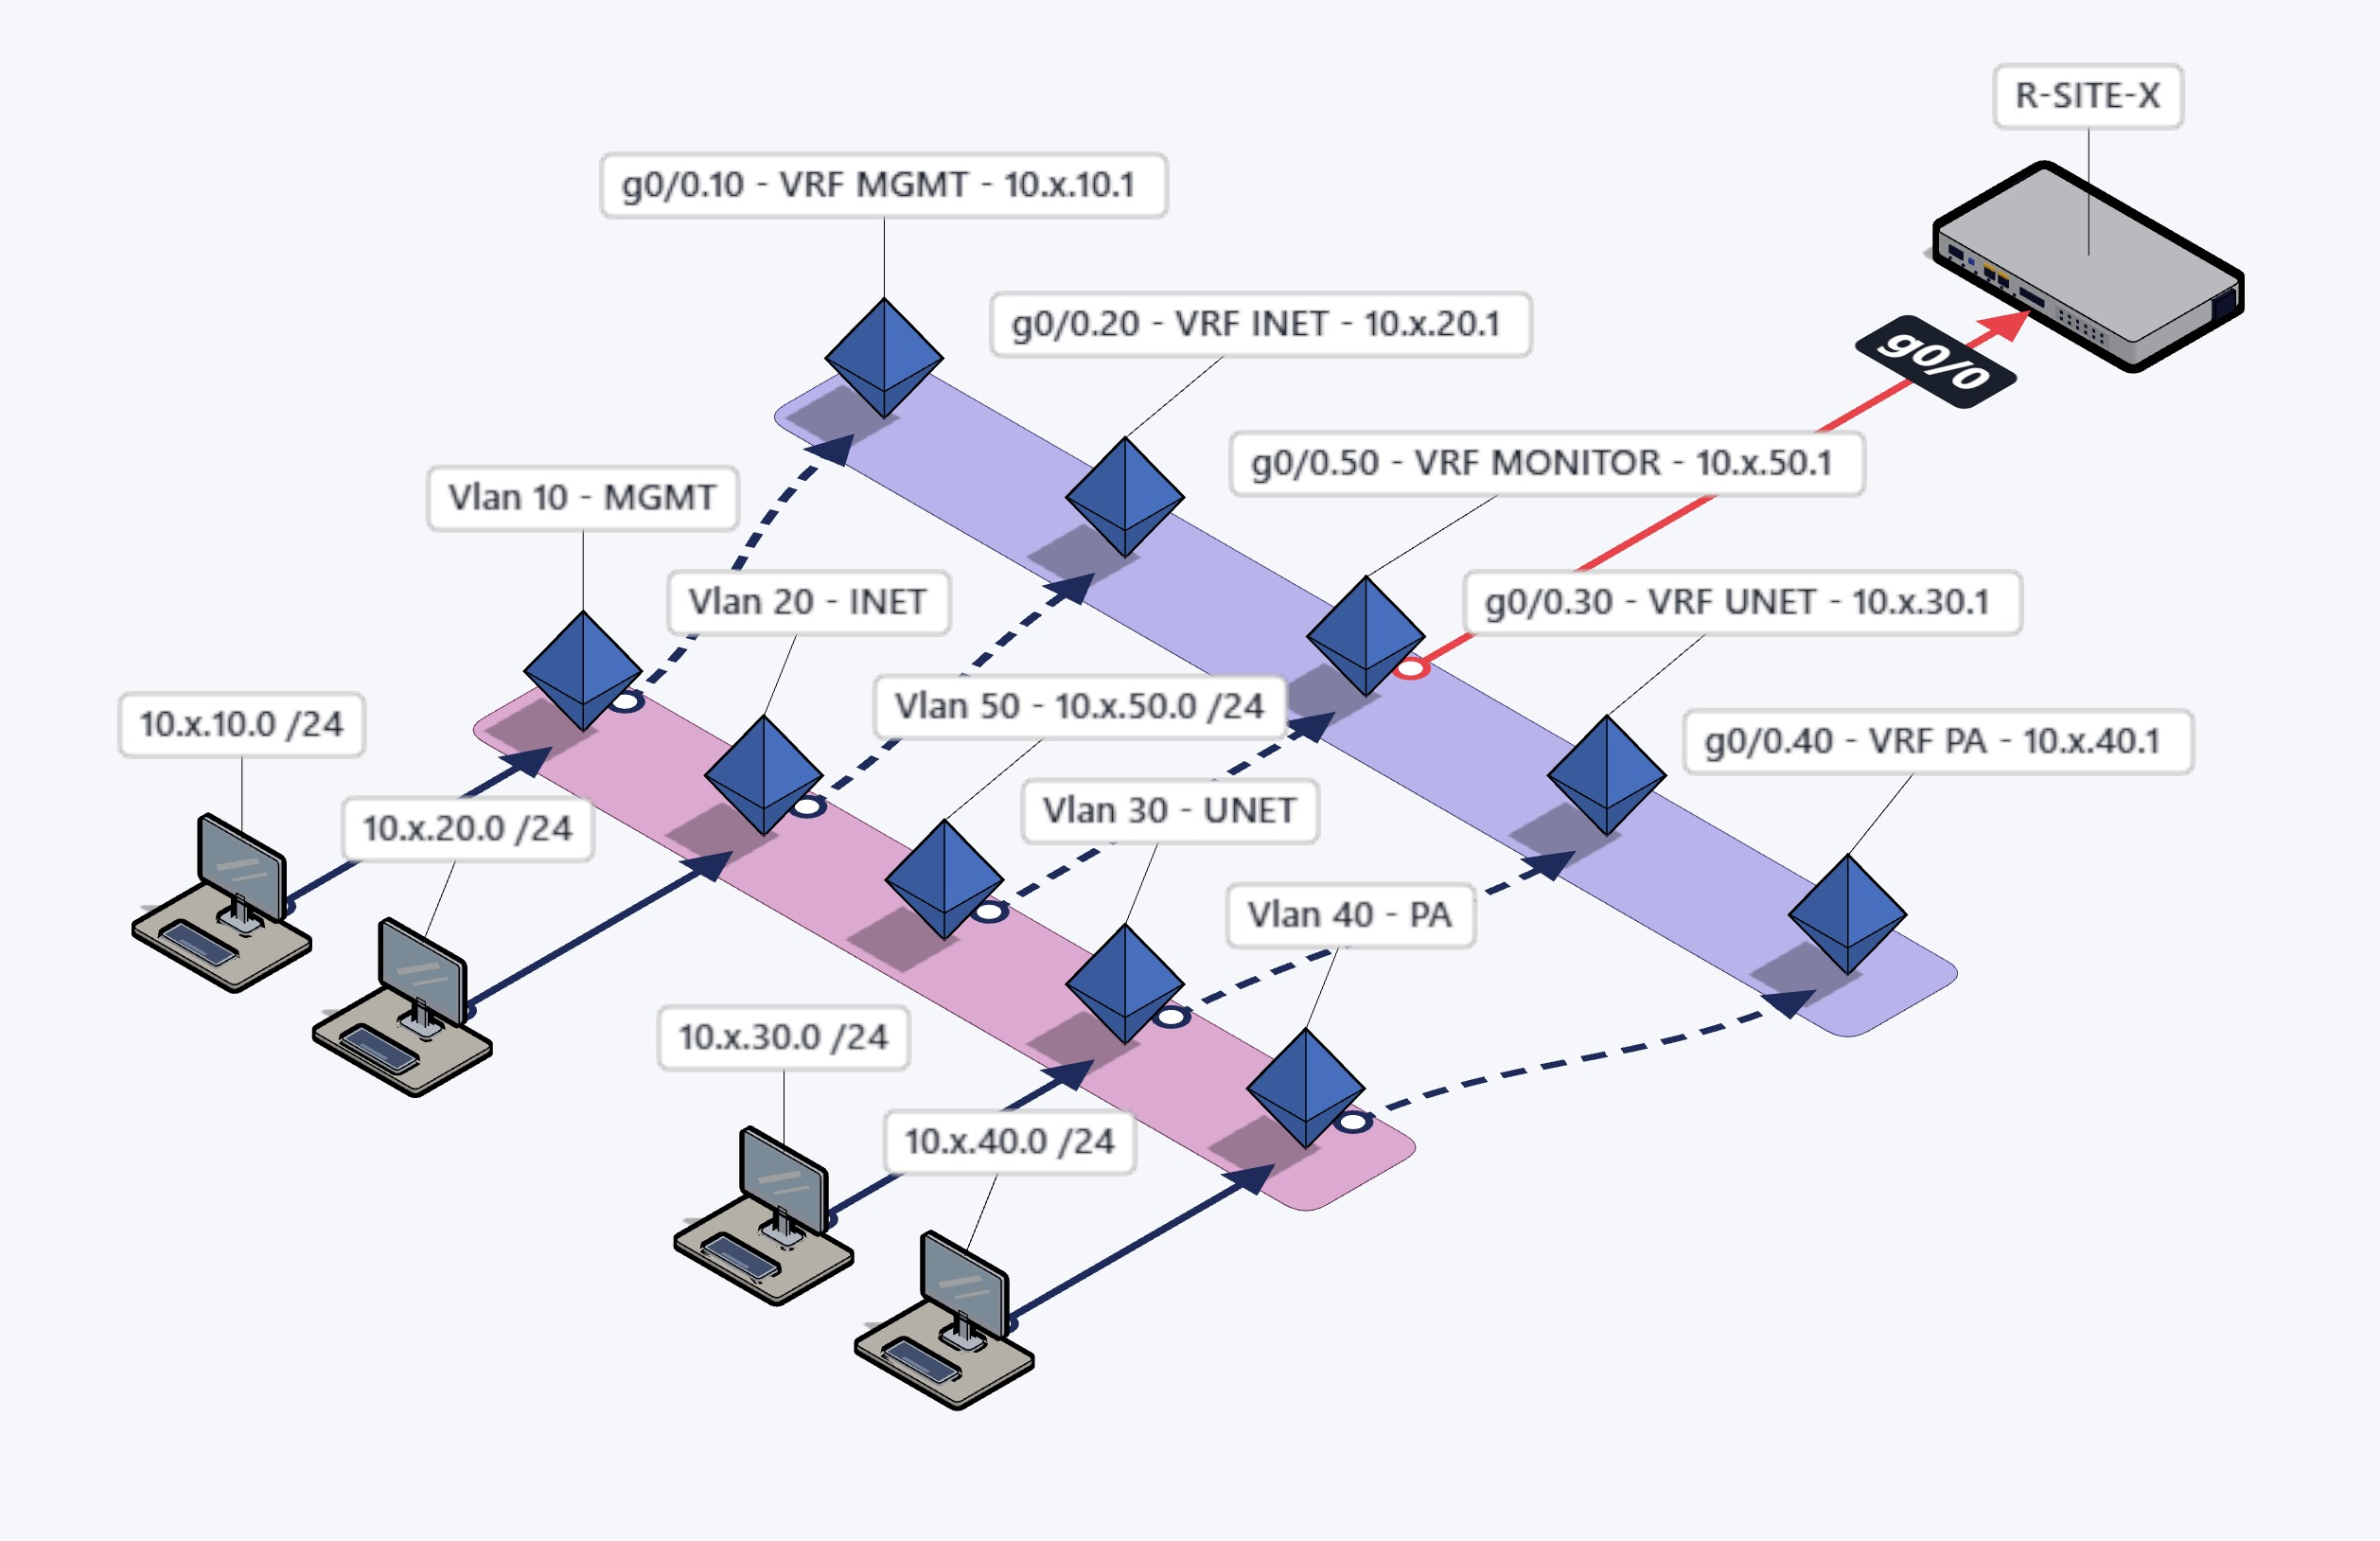
\includegraphics[width=1\textwidth]{../Media/log_ip.jpg}
    \caption{Logisk design for nettverket på lokasjon X.}
    \label{fig:logisk_ip}
\end{figure}
\noindent
BNHQ fikk en annen rolle enn spoke-lokasjonene fordi hubben, sentrale tjenester og WAN-/ISP-tilkoblingen ble samlet her. Dette ga et felles administrasjons- og overvåkningspunkt, men medførte også avhengigheter som måtte vurderes ved bortfall av BNHQ.

\subsection{Nettverkssikkerhet}
Sikkerhetsdesignet bygger på flere lag med tiltak. Tabell \ref{tab:router-security} og \ref{tab:switch-security} oppsummerer mekanismene som er implementert på henholdsvis rutere og svitsjer. Denne delen beskriver derfor hovedsakelig hvordan mekanismene brukes i løsningen og hvilke begrensninger som må tas hensyn til.

\subsubsection{Tilgangskontroll mellom nettverk}
VRF-Lite separerer rutingtabellene, mens trafikkpolicyen i \texttt{FLOW\_POLICY} bestemmer hvilken trafikk som eksplisitt tillates. Generatoren oversetter policyen til extended ACL-er som legges inbound på lokale lag-3-grensesnitt. ACL-ene oppretter ikke ruting mellom VRF-er; eventuell kommunikasjon på tvers av VRF-grenser krever derfor også en kontrollert rutingsmekanisme.

Hver genererte ACL avsluttes med en deny-regel med logging. Dersom \texttt{FLOW\_POLICY} er tom, genereres ingen slike ACL-er, og det må derfor kontrolleres at alle relevante kildesoner er representert i policyen.

\subsubsection{Administrasjon og AAA}
Administrativ tilgang er begrenset til MGMT-nettene. TACACS+ brukes som sentral AAA-tjeneste, mens en lokal bruker fungerer som reserve dersom den sentrale tjenesten er utilgjengelig.

Generatoren konfigurerer autentisering, EXEC-autorisasjon og accounting av EXEC-sesjoner og kommandoer på privilege-nivå 15. Denne generatorversjonen oppretter ikke en egen metodeliste for kommandoautorisasjon, og individuell godkjenning av hver kommando inngår derfor ikke i løsningen. Reserveinnlogging og oppførsel ved bortfall av TACACS+ må verifiseres i test.

\subsubsection{Tilgangskontroll på klientporter}
Utvalgte klientporter bruker IEEE 802.1X med RADIUS. Endepunkter som ikke støtter 802.1X må håndteres gjennom en dokumentert unntakspolicy.

Inter-switch-forbindelser er trusted for DHCP Snooping og DAI, slik at legitim DHCP- og ARP-trafikk fra underliggende svitsjer kan passere. Klientporter forblir untrusted. Dette skillet er viktig for at beskyttelsesmekanismene ikke skal blokkere legitim infrastrukturtrafikk.

\subsubsection{Overvåkning, logging og tidsgrunnlag}
Syslog, SNMPv3 og trafikkspeiling gir sentral synlighet, men trafikkspeilingen er passiv og blokkerer ikke angrep.

Ved ERSPAN mottar HUB SW1 de speilede strømmene og sender dem til en dedikert sensorport. På spoke-lokasjonene speiles inngående klienttrafikk, og SW1 speiler i tillegg trafikk som kommer inn fra ruteren. Inter-switch-trunker speiles ikke for å redusere duplikater. Trafikk som kun går lokalt på HUB SW1 fanges ikke av denne varianten.

NTP-oppsettet gir et felles internt tidsgrunnlag, men generatorversjonen benytter ikke en ekstern autoritativ tidskilde eller reservekilde. Løsningen gir derfor konsistente tidsstempler internt, men korrekt UTC og oppførsel ved bortfall må verifiseres separat.

\subsubsection{Sikkerhetsmekanismer på rutere}
Tabell \ref{tab:router-security} oppsummerer sikkerhetsmekanismene som inngår i ruterdesignet.

\begin{table}[H]
\centering
\caption{Sikkerhetsmekanismer i designet for lokasjonsrutere.}
\vspace{5pt}
\small
\setlength{\tabcolsep}{6pt}
\rowcolors{2}{lightgreen}{white}
\begin{tabular}{>{\raggedright\arraybackslash}p{3.8cm}>{\raggedright\arraybackslash}p{9.9cm}}
\toprule
\rowcolor{tablegreen}
\color{white}\textbf{Mekanisme} & \color{white}\textbf{Funksjon} \\
\midrule
VRF-Lite &
Skiller tjenestenettene i separate rutingtabeller og reduserer muligheten for lateral kommunikasjon. \\
Flow-policy / ACL &
Tillater bare eksplisitt definert trafikk mellom segmentene og blokkerer øvrig trafikk. \\
DMVPN Phase 3 &
Gir skalerbar dynamisk kommunikasjon mellom lokasjoner og muliggjør direkte spoke-to-spoke-shortcuts. \\
IPsec &
Beskytter utvalgte DMVPN-overlay mot avlytting og manipulering. \\
SSH v2 &
Gir kryptert fjernadministrasjon av nettverksenhetene. \\
SSH-MGMT-ONLY ACL &
Begrenser administrativ tilgang til godkjente MGMT-nett. \\
AAA / TACACS+ &
Gir innloggingsautentisering, EXEC-autorisasjon og accounting av sesjoner og kommandoer på nivå 15. \\
Syslog &
Sender system- og sikkerhetshendelser til sentral loggtjeneste. \\
NTP &
Gir nettverksenhetene et felles tidsgrunnlag. \\
No IP redirects &
Hindrer ruteren i å påvirke klientenes ruting ved hjelp av ICMP Redirect. \\
No Proxy ARP &
Hindrer ruteren i å svare på ARP på vegne av andre systemer. \\
EIGRP passive-interface &
Begrenser etablering av EIGRP-naboskap til grensesnitt der rutingprotokollen faktisk skal benyttes. \\
\bottomrule
\end{tabular}
\rowcolors{1}{}{}
\label{tab:router-security}
\end{table}

\subsubsection{Sikkerhetsmekanismer på svitsjer}
Tabell \ref{tab:switch-security} oppsummerer sikkerhetsmekanismene som inngår i svitsjdesignet.

\begin{table}[H]

\centering
\caption{Sikkerhetsmekanismer i designet for svitsjer.}
\vspace{5pt}
\small

\setlength{\tabcolsep}{6pt}

\rowcolors{2}{lightgreen}{white}

\begin{tabular}{
    >{\raggedright\arraybackslash}p{3.8cm}
    >{\raggedright\arraybackslash}p{9.9cm}
}

\toprule

\rowcolor{tablegreen}
\color{white}\textbf{Mekanisme} &
\color{white}\textbf{Funksjon} \\

\midrule

DHCP Snooping &
Blokkerer uautoriserte DHCP-servere og etablerer bindinger mellom port, IP-adresse og MAC-adresse. \\

Dynamic ARP Inspection &
Validerer ARP-trafikk mot gyldige IP--MAC-bindinger og reduserer ARP-spoofing. \\

IP Source Guard &
Kontrollerer at trafikk inn på en aksessport benytter en gyldig kilde-IP-adresse. \\

Port Security &
Begrenser hvilke og hvor mange MAC-adresser som kan benyttes på en aksessport. \\

BPDU Guard &
Stenger edge-porter dersom de mottar BPDU-er. \\

Root Guard &
Hindrer uautoriserte downstream-svitsjer i å overta rollen som STP-root. \\

Loop Guard &
Reduserer risikoen for lag-2-løkker som følge av unidireksjonelle forbindelsesfeil. \\

Blackhole VLAN &
Plasserer ubrukte porter i et VLAN som ikke transporterer produksjonstrafikk. \\

Shutdown av ubrukte porter &
Hindrer fysisk nettverkstilgang gjennom porter som ikke er i bruk. \\

Trunk allow-list &
Begrenser hvilke VLAN som kan transporteres over trunkforbindelser. \\

SSH v2 &
Gir kryptert administrasjon av svitsjene. \\

AAA / TACACS+ &
Gir sentral kontroll av administrativ innlogging. \\

Syslog &
Sender hendelser fra svitsjene til sentral loggtjeneste. \\

NTP &
Sikrer konsistente tidsstempler på tvers av nettverksenhetene. \\

SPAN/RSPAN/
ERSPAN &
Gjør relevant nettverkstrafikk tilgjengelig for sentral IDS-analyse. \\

EtherChannel &
Gir redundans og økt tilgjengelighet på forbindelser mellom svitsjer. \\

\bottomrule

\end{tabular}

\rowcolors{1}{}{}

\label{tab:switch-security}

\end{table}


\subsection{Standardisering og konfigurasjonsgenerator}

Konfigurasjonsgeneratoren bruker ett felles Excel-grunnlag for å produsere standardiserte konfigurasjoner for rutere og svitsjer. Excel-filen beskriver ønsket nettverksdesign, mens generatoren oversetter dette til enhetskonfigurasjon og filer som kan brukes videre av Ansible. Dette reduserer manuelt arbeid og gjør det enklere å bruke samme konfigurasjonsprinsipper på tvers av lokasjoner.

\begin{table}[H]
    \centering
    \caption{Oversikt over hva konfigurasjonsgeneratoren genererer.}
    \label{tab:generator-output}
    \small
    \renewcommand{\arraystretch}{1.35}
    \setlength{\tabcolsep}{5pt}
    \rowcolors{2}{lightgreen}{white}
    \begin{tabular}{
        >{\raggedright\arraybackslash}p{2.8cm}
        >{\raggedright\arraybackslash}p{12cm}
    }
        \toprule
        \rowcolor{tablegreen}
        \color{white}\textbf{Område} &
        \color{white}\textbf{Generert innhold} \\
        \midrule

        Ruter &
        VRF-Lite, grensesnitt og gateway-adresser, DHCP, QoS, \texttt{FLOW\_POLICY}-ACL-er, DMVPN, EIGRP, valgfri IPsec, NAT/PAT og ruting. \\
        \addlinespace[2pt]

        Svitsjer &
        VLAN, access- og trunkporter, EtherChannel, portsikkerhet, DHCP Snooping, DAI, IP Source Guard, STP-beskyttelse, RADIUS/802.1X og SPAN/RSPAN/ERSPAN. \\
        \addlinespace[2pt]

        Administrasjon &
        SSH/SCP, lokal administrasjonsbruker, TACACS+, syslog, NTP og valgfri SNMPv3. \\
        \addlinespace[2pt]

        RADIUS &
        FreeRADIUS-klienter med svitsjenes management-adresser. \\
        \addlinespace[2pt]

        Ansible &
        \texttt{inventory.ini}, \texttt{legacy\_ssh.cfg}, enhets- og SSH/SCP-konfigurasjoner samt utrullingsplaybook. \\
        \addlinespace[2pt]

        Dokumentasjon / filer &
        Tekstfiler og JSON-modeller for ruter- og svitsjkonfigurasjoner per site og enhet. \\

        \bottomrule
    \end{tabular}
    \rowcolors{1}{}{}
\end{table}

Excel-arbeidsboken er strukturert slik at nettverksdata og valg som varierer mellom lokasjoner kan endres uten at Python-koden må skrives om. En detaljert oversikt over forventede tabeller, felter og betingede parametere er derfor lagt til som vedlegg.

\textcolor{red}{\textbf{Se vedlegg XXX for forventet datagrunnlag og struktur i Excel-arbeidsboken.}}

\subsection{Utrulling, sikkerhetskopi og gjenoppretting}

\subsubsection{Utrulling }
Diagramet under viser arbeidsflyten for utrulling av konfigurasjoner fra generering til verifikasjon og lagring i \texttt{startup-config}.
\begin{figure}[H]
\centering
\includegraphics[width=1\textwidth]{../../Media/init_pdf.pdf}
\caption{Arbeidsflyt for utrulling av konfigurasjoner}
\label{fig:utrulling_workflow}
\end{figure}
\noindent
Dersom SSH ikke er tilgjengelig, er \texttt{copy and paste} versjon av konfigurasjonene også tilgjengelig.

\subsubsection{Sikkerhetskopi}
Diagrammet under viser arbeidsflyten for sikkerhetskopiering av konfigurasjoner før endringer (K8).
\begin{figure}[H]
\centering
\includegraphics[width=1\textwidth]{../../Media/backup_pdf.pdf}
\caption{Arbeidsflyt for sikkerhetskopiering av konfigurasjoner}
\label{fig:backup_workflow}
\end{figure}

\subsubsection{Gjenoppretting}
Diagrammet under viser arbeidsflyten for gjenoppretting av konfigurasjoner fra sikkerhetskopi (K8).
\begin{figure}[H]
\centering
\includegraphics[width=1\textwidth]{../../Media/restore_pdf.pdf}
\caption{Arbeidsflyt for gjenoppretting av konfigurasjoner}
\label{fig:restore_workflow}
\end{figure}

\subsection{Fysiske og organisatoriske tiltak}
K7 kan ikke løses med nettverkskonfigurasjon alene. Ubrukte uttak bør deaktiveres, portprofiler dokumenteres og nettverksutstyr plasseres skjermet. I tillegg må rom, uttak og brukergrupper kartlegges slik at soneinndeling (K1) og porttilgang (K3) bygger på faktiske operative behov.

Segmentering løser ikke risikoen for at en kompromittert Internett-klient kan ta opp samtaler i et sensitivt rom. Klientplassering, endepunktsikring og bruk av flyttbare lagringsmedier må derfor avklares med S6 og sikkerhetsfunksjonen. Designet gjelder det UGRADERTE nettet og innebærer ingen godkjenning for behandling av gradert informasjon.

Før overlevering må ansvar for brukerforvaltning, rettigheter, varsler, oppdateringer og hendelseshåndtering være avklart. Opplæring og driftsprosedyrer er en del av dokumentasjonsbehovet i F5. Ressursbruken må samtidig vurderes mot F1, og uavklarte forhold må synliggjøres for S6.

\subsection{Operative konsekvenser}
Segmenteringen gjør at kommunikasjon som tidligere fungerte fritt i det flate nettet, ikke lenger tillates automatisk. Nødvendige applikasjons- og tjenesteflyter må derfor være identifisert og lagt inn i trafikkpolicyen før produksjonssetting.

Feil i ACL-er, DHCP-beskyttelse, STP eller ruting kan føre til bortfall av tjenester. Konfigurasjonen bør derfor valideres i et separat testmiljø før den tas i produksjon.

Standardiseringen skal redusere driftsbelastningen (F1), men sentrale tjenester gir også nye vedlikeholdsoppgaver. Gevinsten ved AAA, logging, NTP og konfigurasjonsgenerering må derfor veies mot arbeidet med servere, sertifikater, brukere og overvåkningsregler. At tjenestene er sentralisert, dokumenterer ikke alene at ressursbehovet blir lavere.

DMVPN Phase 3 gjør det mulig å legge til nye spoke-lokasjoner uten at det må opprettes separate punkt-til-punkt-tunneler mellom alle lokasjoner. Dette forbedrer skalerbarheten sammenlignet med en tradisjonell full-mesh av statiske GRE-tunneler.


\clearpage

\section{Diskusjon}

Diskusjonen vurderer designets konsekvenser og begrensninger innenfor F1--F6. 

\textcolor{red}{\textbf{Vedlegg \ref{sec:vedlegg-testmatrise} må legges inn før innlevering.}}

\subsection{Ruting, utstyr og adresseplan}

VRF-Lite og separate DMVPN-overlay gir ende-til-ende segmentering uten at leverandørens lag-3-VPN må rekonfigureres. Rapporterte labresultater støtter at segmentering og ruting fungerte, også ved testede brudd. Phase 3 gir samtidig bedre skalerbarhet enn statiske punkt-til-punkt-tunneler fordi nye spoke-lokasjoner kan legges til uten full mesh-konfigurasjon, mens dataplanet kan etablere direkte spoke-to-spoke-forbindelser.

Adresseplanen \texttt{10.X.Y.0/24} prioriterer enkel drift fremfor maksimal adresseutnyttelse. /24-nett er større enn nødvendig for flere tjenester, men site og tjeneste kan leses direkte fra adressen, noe som forenkler dokumentasjon og feilsøking.

Bruk av eksisterende Cisco-utstyr reduserer behovet for nyanskaffelser, men gjør plattformkompatibilitet viktig. Generatoren støtter flere syntaksvalg, men endelig konfigurasjon må fortsatt valideres mot IOS-versjonen på produksjonsutstyret.

\subsection{Kryptering og sikkerhet}

Sikkerheten er avhengig av at flere lag virker sammen. VRF-er begrenser rutingsdomenene, ACL-er styrer tillatte flyter, og IPsec beskytter overlay der konfidensialitet og integritet kreves. Testingen viste at filtrering og IPsec fungerte etter designet. Krypteringen reduserer samtidig behovet for å stole på underliggende transportinfrastruktur som eFP ikke administrerer.

Den viktigste operative risikoen ligger derfor ikke i en enkelt mekanisme, men i feil konfigurasjon av grensene mellom dem. Feil trusted/untrusted-rolle kan for eksempel svekke beskyttelsen på klientporter eller blokkere legitim infrastrukturtrafikk. Standardisert generering reduserer risikoen for slike avvik, men erstatter ikke kontroll av kabling, portroller og generert konfigurasjon.

\subsection{Tilgangskontroll og autonomi}

TACACS+ og RADIUS gir sentral kontroll, men gjør samtidig lokasjonene avhengige av tjenester på BNHQ. Testene viste at TACACS+-accounting og lokal reservetilgang fungerte som forventet, og at en eksplisitt avvisning fra en tilgjengelig TACACS+-server ikke ble omgått av lokal fallback. Ved RADIUS-bortfall ble det heller ikke gitt utilsiktet ny klienttilgang. Dette bevarer lokal administrasjon ved bortfall, men nye klienter kan miste nettverkstilgang når RADIUS er utilgjengelig. Autonomien gjelder derfor ikke alle tjenester.

802.1X ble også testet sammen med DHCP Snooping, DAI og IP Source Guard. Det er viktig fordi sikkerhetsmekanismer som fungerer isolert kan påvirke hverandre når de brukes samtidig.

Automatisert utrulling har en tilsvarende oppstartsavhengighet: en helt ukonfigurert enhet er ikke tilgjengelig for Ansible. SSH/SCP-grunnkonfigurasjon og en midlertidig konfigurasjonssvitsj brukes derfor under staging før full konfigurasjon lastes inn. Dette gjør førstegangsoppsettet mer repeterbart og mindre avhengig av at produksjonsruting allerede finnes.

\subsection{Redundans og skalerbarhet}

EtherChannel gir lokal toleranse for brudd i en fysisk forbindelse, og dette ble verifisert i lab. Løsningen har likevel ikke full redundans. BNHQ er fortsatt sentral for NHRP, Internett, administrasjon og flere fellestjenester, selv om DMVPN Phase 3 kan gi direkte spoke-to-spoke-trafikk.

Sentraliseringen forenkler drift, men samler også avhengigheter. Dersom tilgjengelighetskravene økes, bør redundante servere, alternativ hub eller reserveforbindelser vurderes. Innenfor prosjektets ramme om å unngå større nyanskaffelser er dagens løsning et kompromiss mellom robusthet, kompleksitet og ressursbruk.

QoS reduserer konsekvensen av kø ved belastning, men skaper ikke mer kapasitet. Den faktiske brukeropplevelsen vil derfor fortsatt avhenge av tilgjengelig WAN-båndbredde og trafikkmønster.

\subsection{Sikkerhetsovervåkning, logging og arkitektur}

Sentral syslog, SNMPv3, NTP og lokal trafikkspeiling ble verifisert i lab og gir et bedre grunnlag for feilsøking og hendelsesanalyse enn i det opprinnelige nettet.

ERSPAN kunne ikke testes ende-til-ende fordi labutstyret manglet støtte, og må verifiseres på produksjonsutstyret. Lokal SPAN og speilingslogikken ble testet. Generatorens støtte for SPAN, RSPAN og ERSPAN gir alternativer som må vurderes mot endelig topologi.

Valgt metode må vurderes mot kapasitet, blindsoner og duplikater. Trafikkspeiling er dessuten passiv og må sees som et supplement til segmentering, tilgangskontroll og filtrering, ikke som en mekanisme som i seg selv stopper angrep.

\subsection{Ikke-tekniske aspekter}

Nettverksdesign kan ikke alene håndtere fysisk risiko. Et deaktivert uttak har begrenset verdi dersom en bruker kan flytte kabelen til et annet ubeskyttet uttak, og segmentering beskytter ikke mot en kompromittert klient som fysisk befinner seg i et sensitivt rom. Plassering av klienter og nettverksutstyr må derfor inngå i den samlede sikkerhetsvurderingen.

Løsningen innfører også nye driftsoppgaver knyttet til AAA, RADIUS, logging, NTP, overvåkning, brukere og automatisering. Standardisering og sentralisering reduserer manuelt arbeid og konfigurasjonsavvik, men dokumenterer ikke i seg selv at total ressursbruk blir lavere. Dette må vurderes over tid mot kravet i F1.

Konfigurasjonsgeneratoren reduserer personavhengighet, men gjør Excel-grunnlaget til en viktig del av konfigurasjonsforvaltningen. En feil i datagrunnlaget kan ellers bli reprodusert på flere enheter. Testing, versjonskontroll, sikkerhetskopi og gjenoppretting er derfor viktige deler av løsningen og gjør det enklere for senere kontingenter å overta driften.

\subsection{Test og verifikasjon}

De rapporterte labresultatene støtter hovedfunksjonene, men dokumenterer ikke uten videre kravoppfyllelse i produksjonsnettet. Testmatrisen vedlegges som dokumentasjon på gjennomførte tester, testbetingelser, akseptkriterier og observerte resultater (Vedlegg \ref{sec:vedlegg-testmatrise}).

Før produksjonssetting bør det gjennomføres en siste ende-til-ende-verifikasjon av faktisk utstyr og transportforbindelse. Den bør særlig bekrefte ERSPAN eller valgt alternativ speilingsmetode, MTU gjennom GRE/IPsec, oppførsel ved bortfall av sentrale tjenester og at nødvendige tjenesteflyter er representert i \texttt{FLOW\_POLICY}. Dette gir et tydeligere grunnlag for S6 sin aksept av gjenværende operativ risiko.

\clearpage

\section{Konklusjon}
Designet vi har presentert viser hvordan bataljonsstridsgruppens ugraderte nettverk kan organiseres i adskilte sikkerhetssoner med kontrollert kommunikasjon mellom tjenestene og lokasjonene. Dette, sammen med tilgangskontroll, sikker administrasjon og logging samt gjennomføring av de foreslåtte fysiske og organisatoriske tiltakene, vil redusere risikoen knyttet til det flate nettverket.

Laboratorietestene viser at sentrale deler av designet fungerer etter hensikten. Dette gjelder segmentering og ruting, filtrering, kryptert transport, tilgangskontroll og logging. Derimot har ikke alle deler av designet blitt testet. ERSPAN er ikke verifisert ende til ende, og plattformspesifikk IOS-kompatibilitet må kontrolleres mot det endelige utstyret. Det må også vurderes om løsningen kan driftes innenfor dagens ressursramme.

Designet gir dermed S6 et grunnlag for videre verifikasjon og beslutning om rekonfigurasjon. Før endringer i produksjonsnettet bør de uavklarte forholdene testes på faktisk utstyr og transportforbindelse, det bør bekreftes at eksisterende tjenester opprettholdes, og gjenværende operativ risiko bør vurderes og aksepteres av S6.


\clearpage

%TC:ignore
\phantomsection
\printbibliography[heading=bibintoc,title={Referanser}]
\clearpage

\phantomsection
\section*{Vedlegg}
\addcontentsline{toc}{section}{Vedlegg}
\label{sec:vedlegg}
\appendix

\section{Beregning av QoS-andeler}
\label{sec:vedlegg-qos}
For trafikkklasse $i$ beregner generatoren minimumsandelen som
\[
 B_i=\frac{P_i}{\sum_j P_j}\cdot75\%,
\]
der $P_i$ er klassens prioriteringsvekt. Andelene avrundes først ned til heltall. Resterende prosentpoeng fordeles til klassene med størst desimalrest; ved lik rest prioriteres høyere vekt. De tildelte andelene summerer dermed til 75 prosent.

\section{Testmatrise og testbevis}
\label{sec:vedlegg-testmatrise}
\textbf{Må ferdigstilles før innlevering.} Testmatrisen og testbevisene var ikke inkludert i rapportmappen som ble revidert. Sett inn faktisk dokumentasjon med kobling til K1--K8, testbetingelser, akseptkriterier, observerte resultater og avvik. Påstander om gjennomførte tester i hovedteksten må kontrolleres mot denne dokumentasjonen.

\section{Datagrunnlag for konfigurasjonsgeneratoren}
\label{sec:vedlegg-excel}
\textbf{Må ferdigstilles før innlevering.} Sett inn den planlagte oversikten over Excel-arbeidsbokens tabeller, felter og betingede parametere. Det opprinnelige utkastet henviste til dette vedlegget, men inneholdt ikke selve oversikten.

\section{Security onion konfigurasjon}
\label{sec:vedlegg-seconi}
Må ferdigstilles før innlevering. Beskriv hvordan Security Onion settes opp, inkludert installasjonen som brukes i CyberOps.

\section{Link til git repository}
\label{sec:vedlegg-git}
Må ferdigstilles før innlevering. Sett inn lenke til git repository som inneholder prosjektets kildekode og relevant dokumentasjon.
%TC:endignore

\end{document}
